% Options for packages loaded elsewhere
\PassOptionsToPackage{unicode}{hyperref}
\PassOptionsToPackage{hyphens}{url}
\PassOptionsToPackage{dvipsnames,svgnames,x11names}{xcolor}
%
\documentclass[
  letterpaper,
  DIV=11,
  numbers=noendperiod]{scrartcl}

\usepackage{amsmath,amssymb}
\usepackage{iftex}
\ifPDFTeX
  \usepackage[T1]{fontenc}
  \usepackage[utf8]{inputenc}
  \usepackage{textcomp} % provide euro and other symbols
\else % if luatex or xetex
  \usepackage{unicode-math}
  \defaultfontfeatures{Scale=MatchLowercase}
  \defaultfontfeatures[\rmfamily]{Ligatures=TeX,Scale=1}
\fi
\usepackage{lmodern}
\ifPDFTeX\else  
    % xetex/luatex font selection
  \setmainfont[]{Times New Roman}
\fi
% Use upquote if available, for straight quotes in verbatim environments
\IfFileExists{upquote.sty}{\usepackage{upquote}}{}
\IfFileExists{microtype.sty}{% use microtype if available
  \usepackage[]{microtype}
  \UseMicrotypeSet[protrusion]{basicmath} % disable protrusion for tt fonts
}{}
\makeatletter
\@ifundefined{KOMAClassName}{% if non-KOMA class
  \IfFileExists{parskip.sty}{%
    \usepackage{parskip}
  }{% else
    \setlength{\parindent}{0pt}
    \setlength{\parskip}{6pt plus 2pt minus 1pt}}
}{% if KOMA class
  \KOMAoptions{parskip=half}}
\makeatother
\usepackage{xcolor}
\setlength{\emergencystretch}{3em} % prevent overfull lines
\setcounter{secnumdepth}{-\maxdimen} % remove section numbering
% Make \paragraph and \subparagraph free-standing
\ifx\paragraph\undefined\else
  \let\oldparagraph\paragraph
  \renewcommand{\paragraph}[1]{\oldparagraph{#1}\mbox{}}
\fi
\ifx\subparagraph\undefined\else
  \let\oldsubparagraph\subparagraph
  \renewcommand{\subparagraph}[1]{\oldsubparagraph{#1}\mbox{}}
\fi


\providecommand{\tightlist}{%
  \setlength{\itemsep}{0pt}\setlength{\parskip}{0pt}}\usepackage{longtable,booktabs,array}
\usepackage{calc} % for calculating minipage widths
% Correct order of tables after \paragraph or \subparagraph
\usepackage{etoolbox}
\makeatletter
\patchcmd\longtable{\par}{\if@noskipsec\mbox{}\fi\par}{}{}
\makeatother
% Allow footnotes in longtable head/foot
\IfFileExists{footnotehyper.sty}{\usepackage{footnotehyper}}{\usepackage{footnote}}
\makesavenoteenv{longtable}
\usepackage{graphicx}
\makeatletter
\def\maxwidth{\ifdim\Gin@nat@width>\linewidth\linewidth\else\Gin@nat@width\fi}
\def\maxheight{\ifdim\Gin@nat@height>\textheight\textheight\else\Gin@nat@height\fi}
\makeatother
% Scale images if necessary, so that they will not overflow the page
% margins by default, and it is still possible to overwrite the defaults
% using explicit options in \includegraphics[width, height, ...]{}
\setkeys{Gin}{width=\maxwidth,height=\maxheight,keepaspectratio}
% Set default figure placement to htbp
\makeatletter
\def\fps@figure{htbp}
\makeatother

\usepackage{hyperref}

% customize figure references
\renewcommand{\figureautorefname}{Fig.}

% toggle line numbers
\usepackage{lineno}
% \linenumbers

% toggle spacing
\usepackage{setspace}
\singlespacing
% \doublespacing

% Hawaiian language characters
% https://tex.stackexchange.com/questions/424535/how-to-type-a-proper-hawai%CA%BBian-%CA%BBokina
\usepackage[utf8]{inputenc}
\usepackage{newunicodechar,graphicx}

\DeclareRobustCommand{\okina}{%
  \raisebox{\dimexpr\fontcharht\font`A-\height}{%
    \scalebox{0.8}{`}%
  }%
}
\newunicodechar{ʻ}{\okina}

% make better hyphen for numeric ranges, \numrange{}{}
\usepackage[detect-none]{siunitx}
\sisetup{range-phrase = \text{--}}
\usepackage{booktabs}
\usepackage{longtable}
\usepackage{array}
\usepackage{multirow}
\usepackage{wrapfig}
\usepackage{float}
\usepackage{colortbl}
\usepackage{pdflscape}
\usepackage{tabu}
\usepackage{threeparttable}
\usepackage{threeparttablex}
\usepackage[normalem]{ulem}
\usepackage{makecell}
\usepackage{xcolor}
\KOMAoption{captions}{tableheading}
\usepackage{fancyhdr}
\pagestyle{fancy}
\fancyhead[C]{Triplett \textit{et al.} — \textit{American Journal of Botany} 2024 – Appendix S1}
\addtokomafont{disposition}{\rmfamily}
\RedeclareSectionCommand[
  font=\normalfont\Large]{section}
\RedeclareSectionCommand[
  font=\normalfont\normalsize\bfseries]{subsection}
\RedeclareSectionCommand[
  font=\normalfont\normalsize\itshape]{subsubsection}
\RedeclareSectionCommand[
  font=\normalfont\normalsize]{paragraph}
\makeatletter
\makeatother
\makeatletter
\makeatother
\makeatletter
\@ifpackageloaded{caption}{}{\usepackage{caption}}
\AtBeginDocument{%
\ifdefined\contentsname
  \renewcommand*\contentsname{Table of contents}
\else
  \newcommand\contentsname{Table of contents}
\fi
\ifdefined\listfigurename
  \renewcommand*\listfigurename{List of Figures}
\else
  \newcommand\listfigurename{List of Figures}
\fi
\ifdefined\listtablename
  \renewcommand*\listtablename{List of Tables}
\else
  \newcommand\listtablename{List of Tables}
\fi
\ifdefined\figurename
  \renewcommand*\figurename{Figure}
\else
  \newcommand\figurename{Figure}
\fi
\ifdefined\tablename
  \renewcommand*\tablename{Table}
\else
  \newcommand\tablename{Table}
\fi
}
\@ifpackageloaded{float}{}{\usepackage{float}}
\floatstyle{ruled}
\@ifundefined{c@chapter}{\newfloat{codelisting}{h}{lop}}{\newfloat{codelisting}{h}{lop}[chapter]}
\floatname{codelisting}{Listing}
\newcommand*\listoflistings{\listof{codelisting}{List of Listings}}
\makeatother
\makeatletter
\@ifpackageloaded{caption}{}{\usepackage{caption}}
\@ifpackageloaded{subcaption}{}{\usepackage{subcaption}}
\makeatother
\makeatletter
\@ifpackageloaded{tcolorbox}{}{\usepackage[skins,breakable]{tcolorbox}}
\makeatother
\makeatletter
\@ifundefined{shadecolor}{\definecolor{shadecolor}{rgb}{.97, .97, .97}}
\makeatother
\makeatletter
\makeatother
\makeatletter
\makeatother
\ifLuaTeX
  \usepackage{selnolig}  % disable illegal ligatures
\fi
\IfFileExists{bookmark.sty}{\usepackage{bookmark}}{\usepackage{hyperref}}
\IfFileExists{xurl.sty}{\usepackage{xurl}}{} % add URL line breaks if available
\urlstyle{same} % disable monospaced font for URLs
\hypersetup{
  pdftitle={Appendix S1: Supplemental figures and table},
  colorlinks=true,
  linkcolor={blue},
  filecolor={Maroon},
  citecolor={Blue},
  urlcolor={Blue},
  pdfcreator={LaTeX via pandoc}}

\title{Appendix S1: Supplemental figures and table}
\author{}
\date{}

\begin{document}
\maketitle
\ifdefined\Shaded\renewenvironment{Shaded}{\begin{tcolorbox}[interior hidden, borderline west={3pt}{0pt}{shadecolor}, sharp corners, breakable, boxrule=0pt, enhanced, frame hidden]}{\end{tcolorbox}}\fi

\renewcommand\thefigure{S\arabic{figure}}    
\renewcommand\thetable{S\arabic{table}}    
\renewcommand\theequation{S\arabic{equation}}    
\setcounter{figure}{0}    
\setcounter{table}{0}    
\setcounter{equation}{0}

\begin{landscape}
\begin{longtable}{>{\raggedright\arraybackslash}p{4cm}>{\raggedright\arraybackslash}p{1.5cm}>{\raggedright\arraybackslash}p{1.5cm}rrrrrrr}
\caption{Average traits values among ʻilima leaves at each site.
\(\mathrm{SD}_\text{abaxial}\) is the stomatal density per mm\(^2\) on
the abaxial (lower) surface; \(\mathrm{SD}_\text{adaxial}\) is the
stomatal density per mm\(^2\) on the adaxial (upper) surface;
\(\mathrm{GCL}_\text{abaxial}\) is the guard cell length in \(\mu\)m on
the abaxial (lower) surface; \(\mathrm{GCL}_\text{adaxial}\) is the
guard cell length in \(\mu\)m on the adaxial (upper) surface; Leaf
thickness is the length from upper cuticle to lower cuticle in \(\mu\)m;
\(A\) is the photosynthetic rate in
\(\mu \text{mol CO}_2~\text{m}^{-2}~\text{s}^{-1}\); \(g_\mathrm{sw}\)
is the stomatal conductance to water vapor in
\(\text{mol}~\text{m}^{-2}~\text{s}^{-1}\).}\tabularnewline

\toprule
Site & Island & Habitat & $\mathrm{SD}_\text{abaxial}$ & $\mathrm{SD}_\text{adaxial}$ & $\mathrm{GCL}_\text{abaxial}$ & $\mathrm{GCL}_\text{adaxial}$ & Leaf thickness & $A$ & $g_\text{sw}$\\
\midrule
\cellcolor{gray!6}{Kaloko-Honokōhau national historical park} & \cellcolor{gray!6}{Hawaiʻi} & \cellcolor{gray!6}{coastal} & \cellcolor{gray!6}{412.99} & \cellcolor{gray!6}{92.31} & \cellcolor{gray!6}{14.73} & \cellcolor{gray!6}{20.32} & \cellcolor{gray!6}{189.60} & \cellcolor{gray!6}{17.40} & \cellcolor{gray!6}{0.123}\\
Puakō petroglyph park & Hawaiʻi & coastal & 310.12 & 52.55 & 13.35 & 20.94 & 194.20 & 17.85 & 0.134\\
\cellcolor{gray!6}{Kahuku Point} & \cellcolor{gray!6}{Oʻahu} & \cellcolor{gray!6}{coastal} & \cellcolor{gray!6}{420.43} & \cellcolor{gray!6}{80.80} & \cellcolor{gray!6}{16.23} & \cellcolor{gray!6}{22.77} & \cellcolor{gray!6}{304.24} & \cellcolor{gray!6}{20.88} & \cellcolor{gray!6}{0.155}\\
Kaloko beach & Oʻahu & coastal & 400.27 & 109.03 & 15.69 & 23.26 & 399.54 & 31.28 & 0.314\\
\cellcolor{gray!6}{Kaʻena Point} & \cellcolor{gray!6}{Oʻahu} & \cellcolor{gray!6}{coastal} & \cellcolor{gray!6}{370.14} & \cellcolor{gray!6}{120.34} & \cellcolor{gray!6}{17.61} & \cellcolor{gray!6}{22.89} & \cellcolor{gray!6}{295.82} & \cellcolor{gray!6}{34.77} & \cellcolor{gray!6}{0.336}\\
\addlinespace
Makapuʻu beach & Oʻahu & coastal & 408.28 & 23.18 & 15.99 & 22.03 & 249.71 & 32.87 & 0.349\\
\cellcolor{gray!6}{Hāloa ʻĀina} & \cellcolor{gray!6}{Hawaiʻi} & \cellcolor{gray!6}{montane} & \cellcolor{gray!6}{307.94} & \cellcolor{gray!6}{7.61} & \cellcolor{gray!6}{16.49} & \cellcolor{gray!6}{22.59} & \cellcolor{gray!6}{149.41} & \cellcolor{gray!6}{13.07} & \cellcolor{gray!6}{0.116}\\
Kaʻohe game management area & Hawaiʻi & montane & 270.24 & 13.07 & 14.87 & 21.51 & 183.72 & 12.94 & 0.130\\
\cellcolor{gray!6}{Koaiʻa tree sanctuary} & \cellcolor{gray!6}{Hawaiʻi} & \cellcolor{gray!6}{montane} & \cellcolor{gray!6}{318.58} & \cellcolor{gray!6}{9.55} & \cellcolor{gray!6}{13.89} & \cellcolor{gray!6}{22.86} & \cellcolor{gray!6}{138.89} & \cellcolor{gray!6}{27.88} & \cellcolor{gray!6}{0.358}\\
Hawaiʻi loa ridge & Oʻahu & montane & 329.25 & 115.56 & 17.83 & 21.76 & 205.97 & 21.95 & 0.215\\
\addlinespace
\cellcolor{gray!6}{Mauʻumae Ridge} & \cellcolor{gray!6}{Oʻahu} & \cellcolor{gray!6}{montane} & \cellcolor{gray!6}{298.77} & \cellcolor{gray!6}{138.32} & \cellcolor{gray!6}{16.53} & \cellcolor{gray!6}{20.72} & \cellcolor{gray!6}{162.02} & \cellcolor{gray!6}{24.60} & \cellcolor{gray!6}{0.436}\\
Waʻahila ridge & Oʻahu & montane & 346.75 & 150.26 & 17.76 & 20.61 & 193.33 & 13.96 & 0.194\\
\bottomrule
\end{longtable}
\end{landscape}

\newpage

\begin{figure}
  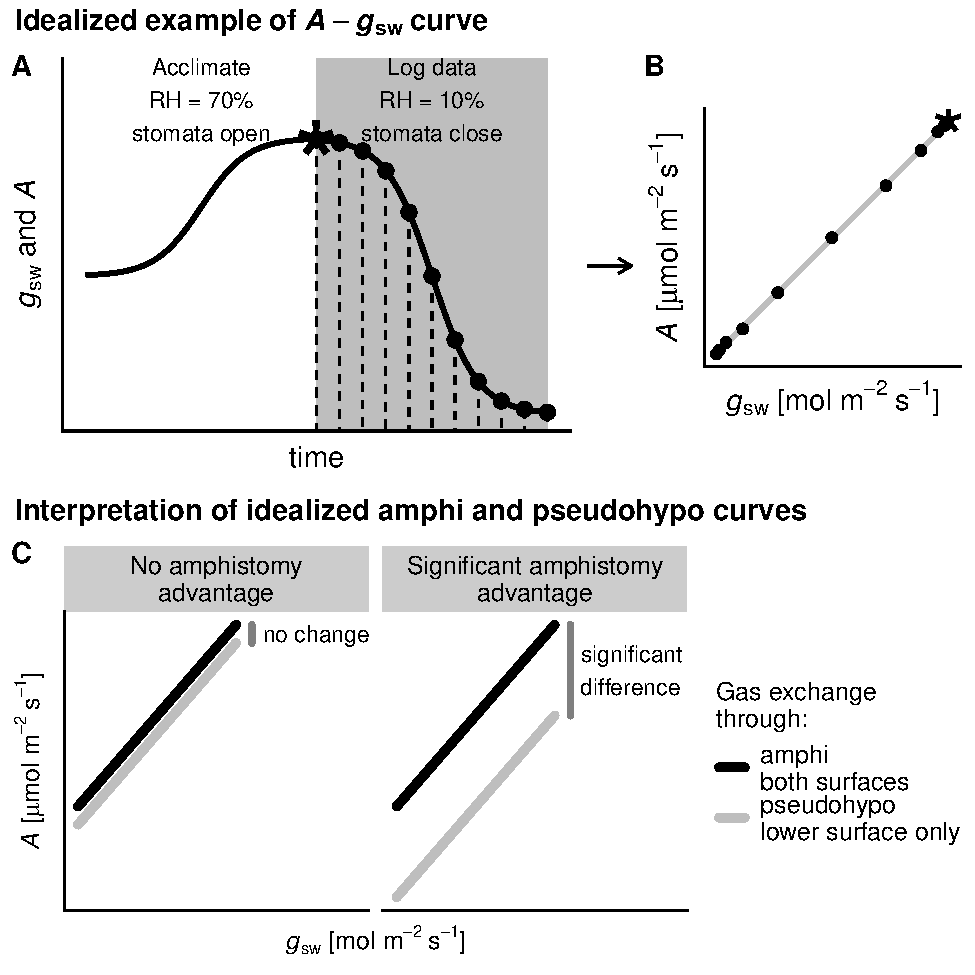
\includegraphics{../figures/ags-curve.pdf}
  \caption{Idealized method for collecting $A \textendash g_\text{sw}$ curves on either amphi or pseudohypo leaves. A) After clamping the leaf into the LI-6800 chamber, it acclimates to high light ($\mathrm{PPFD} = 2000~\mu \text{mol}~\text{m}^{-2}~\text{s}^{-1}$) and humidity ($\mathrm{RH} = 70\%$). This induces stomata to open, increasing $g_\mathrm{sw}$ and $A$ until they reach a maximum. We abruptly lower the chamber humidity to $\approx 10\%$ to close stomata and log data (black points) until $g_\mathrm{sw}$ and $A$ reach their nadir. B) We fit $A \textendash g_\text{sw}$ curves to logged data points. The asterisk in both panels indicates the data point used for maximum $A$ and $g_\mathrm{sw}$. C) $\mathrm{AA}$ is low (left panel) when the photosynthetic rate of an amphi leaf is similar to a pseudohypo leaf at the same total $g_\mathrm{sw}$ ($x$-axes); large $\mathrm{AA}$ (right panel) is indicated when an amphi leaf has a higher photosynthetic rate than a pseudohypo leaf. Abbreviations: $A$ is the photosynthetic rate; $\mathrm{AA}$ is the amphistomy advantage; $g_\mathrm{sw}$ is the stomatal conductance to water vapor; $\mathrm{PPFD}$ is photosynthetic photon flux density; $\mathrm{RH}$ is relative humidity.}
  \label{fig:ags-curve}
\end{figure}

\newpage

\begin{figure}
  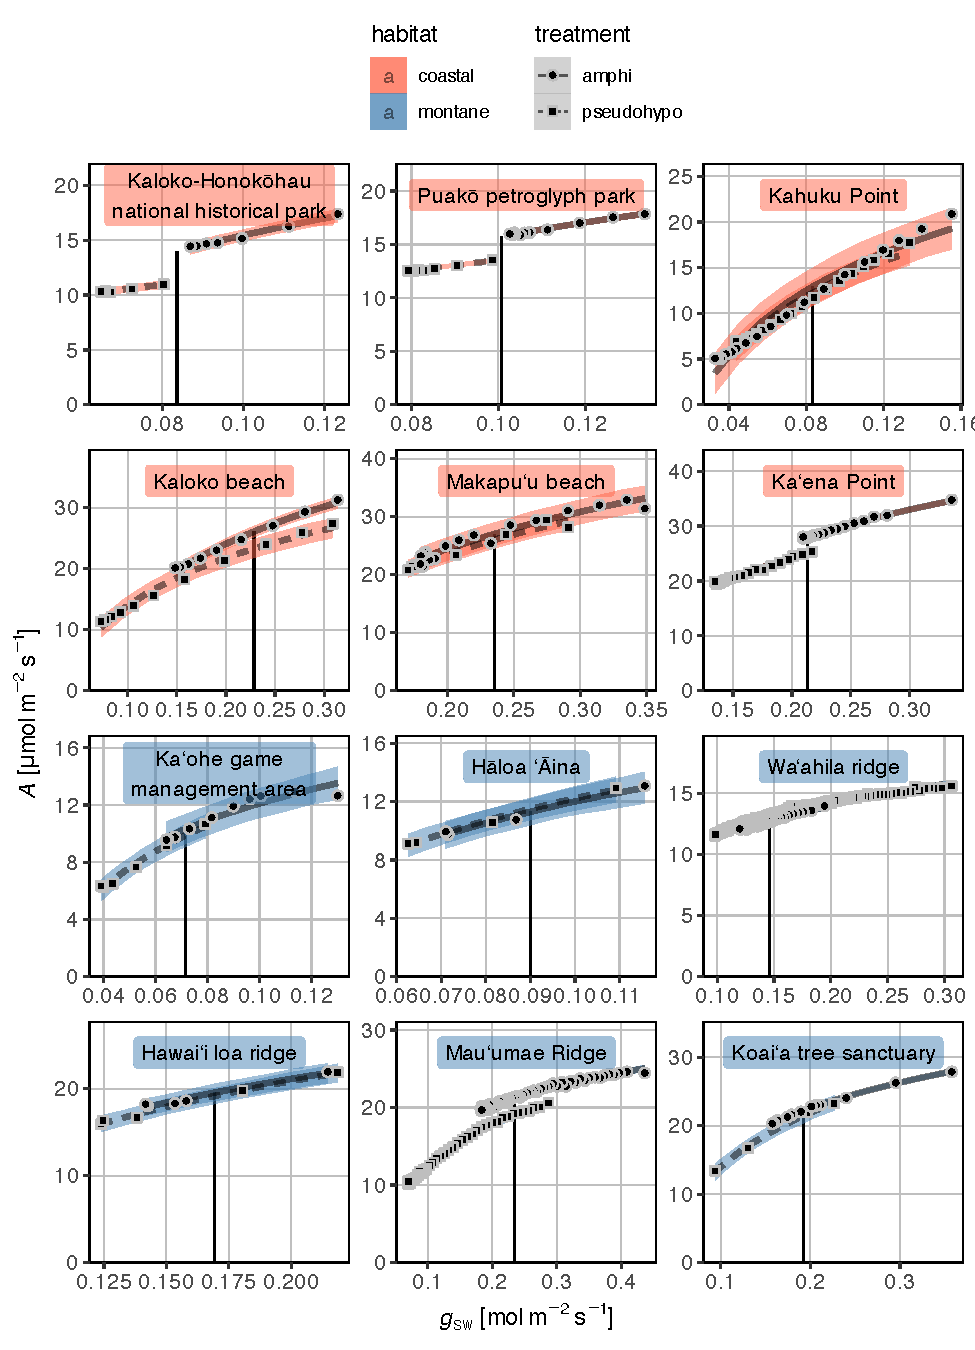
\includegraphics{../figures/licor.pdf}
  \caption{See next page.}
  \label{fig:licor}
\end{figure}

\newpage

\setcounter{figure}{\numexpr\value{figure}-1\relax}

\begin{figure}
  \caption{(Continued from previous page.) Individual $A \textendash g_\mathrm{sw}$ curves used to estimate $\mathrm{AA}$. For each leaf, one per site, we measured $A$ ($y$-axis) over a range of $g_\mathrm{sw}$ ($x$-axis) on the same leaf with two treatments: `amphi' (circles, solid line) leaves were untreated; `pseudohypo' (squares, dashed line) leaves had no conductance through the upper (adaxial) surface. In all coastal (orange) and montane (blue) leaves, we fit generalized additive models and 95\% confidence ribbons to estimate $\mathrm{AA}$ at a $g_\mathrm{sw}$ where the curves overlap (vertical black line). In leaves from Kaloko-Honokōhau national historical park and Puakō petroglyph park, we extrapolated sligtly beyond fitted curves because they did not quite overlap. Symbols: $\mathrm{AA}$, amphistomy advantage; $A$, photosynthetic rate in $\mu \text{mol CO}_2~\text{m}^{-2}~\text{s}^{-1}$; $g_\mathrm{sw}$, stomatal conductance to water vapor in $\text{mol}~\text{m}^{-2}~\text{s}^{-1}$.}
  \label{fig:licor}
\end{figure}

\newpage

\begin{figure}
  \includegraphics{../figures/pp-licor.pdf}
  \caption{Posterior predictions (thin grey lines) from fitted $A \textendash g_\mathrm{sw}$ curves closely match the observed distribution (thick black line), indicating that the statistical model adequately captures variation in the response variable over the measured range. Symbols: $A$, photosynthetic rate in $\mu \text{mol CO}_2~\text{m}^{-2}~\text{s}^{-1}$; $g_\mathrm{sw}$, stomatal conductance to water vapor in $\text{mol}~\text{m}^{-2}~\text{s}^{-1}$.}
  \label{fig:pp-licor}
\end{figure}

\newpage

\begin{figure}
  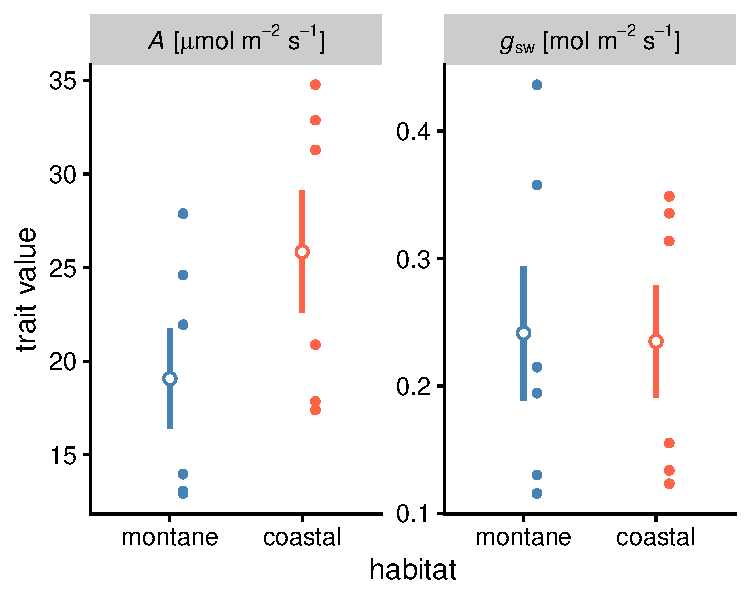
\includegraphics{../figures/habitat-Ags.pdf}
  \caption{The photsynthetic rate (left facet) and stomatal conductance to water vapor (right facet) of montane (blue) and coastal (orange) ʻilima leaves. Each point-interval is the median posterior estimate plus 95\% confidence interval of trait value for that habitat. Smaller points next to each point-interval are the $g_\mathrm{smax,ratio}$ of individual plants, one per site. Symbols: $A$, photosynthetic rate in $\mu \text{mol CO}_2~\text{m}^{-2}~\text{s}^{-1}$; $g_\mathrm{sw}$, stomatal conductance to water vapor in $\text{mol}~\text{m}^{-2}~\text{s}^{-1}$.}
  \label{fig:habitat-Ags}
\end{figure}

\newpage

\begin{figure}
  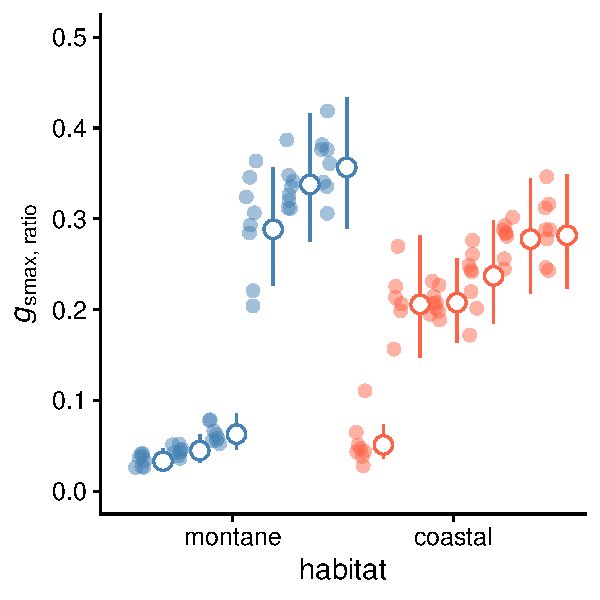
\includegraphics{../figures/habitat-gmaxratio.pdf}
  \caption{The $g_\mathrm{smax,ratio}$ ($y$-axis) of montane (blue) and coastal (orange) ʻilima leaves. Each point-interval is the median posterior estimate plus 95\% confidence interval of $g_\mathrm{smax,ratio}$ for that site. Sites are arranged by habitat and ascending $g_\mathrm{smax,ratio}$ within habitat. Smaller, transparent points next to each point-interval are the $g_\mathrm{smax,ratio}$ of individual plants. Symbols: $g_\mathrm{smax,ratio}$, the ratio of anatomical maximum stomatal conductance to water vapor on the the adaxial surface over the total.}
  \label{fig:habitat-gmaxratio}
\end{figure}



\end{document}
